\documentclass[compress]{beamer}
\usepackage{ifthen,verbatim}

\newcommand{\isnote}{}
\xdefinecolor{lightyellow}{rgb}{1.,1.,0.25}
\xdefinecolor{darkblue}{rgb}{0.1,0.1,0.7}

%% Uncomment this to get annotations
%% \def\notes{\addtocounter{page}{-1}
%%            \renewcommand{\isnote}{*}
%% 	   \beamertemplateshadingbackground{lightyellow}{white}
%%            \begin{frame}
%%            \frametitle{Notes for the previous page (page \insertpagenumber)}
%%            \itemize}
%% \def\endnotes{\enditemize
%% 	      \end{frame}
%%               \beamertemplateshadingbackground{white}{white}
%%               \renewcommand{\isnote}{}}

%% Uncomment this to not get annotations
\def\notes{\comment}
\def\endnotes{\endcomment}

\setbeamertemplate{navigation symbols}{}
\setbeamertemplate{headline}{\mbox{ } \hfill
\begin{minipage}{5.5 cm}
\vspace{-0.75 cm} \small
\end{minipage} \hfill
\begin{minipage}{4.5 cm}
\vspace{-0.75 cm} \small
\begin{flushright}
\ifthenelse{\equal{\insertpagenumber}{1}}{}{Jim Pivarski \hspace{0.2 cm} \insertpagenumber\isnote/\pageref{numpages}}
\end{flushright}
\end{minipage}\mbox{\hspace{0.2 cm}}\includegraphics[height=1 cm]{../cmslogo} \hspace{0.1 cm} \includegraphics[height=1 cm]{../tamulogo} \hspace{0.01 cm} \vspace{-1.05 cm}}

\begin{document}
\begin{frame}
\vfill
\begin{center}
\textcolor{darkblue}{\Large Track-based Alignment of the Muon System}

\vfill
\begin{columns}
\column{0.3\linewidth}
\begin{center}
\large
\textcolor{darkblue}{Jim Pivarski}

\vspace{0.2 cm}
Alexei Safonov

\vspace{0.2 cm}
K\'aroly Banicz
\end{center}

\column{0.5\linewidth}
\begin{center}
\large
Pablo Mart\'inez Ruiz del Arbol

\vspace{0.2 cm}
Francisco Matorras

\vspace{0.2 cm}
Alicia Calder\'on
\vspace{0.2 cm}

\end{center}
\end{columns}

\begin{columns}
\column{0.3\linewidth}
\begin{center}
\scriptsize
{\it Texas A\&M University and US-CMS}
\end{center}
\column{0.5\linewidth}
\begin{center}
\scriptsize
{\it IFCA and INFN}
\end{center}
\end{columns}

\vfill
23 September, 2008

\end{center}
\end{frame}

%% \begin{notes}
%% \item This is the annotated version of my talk.
%% \item If you want the version that I am presenting, download the one
%% labeled ``slides'' on Indico (or just ignore these yellow pages).
%% \item The annotated version is provided for extra detail and a written
%% record of comments that I intend to make orally.
%% \item Yellow notes refer to the content on the {\it previous} page.
%% \item All other slides are identical for the two versions.
%% \end{notes}

\begin{frame}
\small
\frametitle{Intro and Overview for this talk}
\begin{itemize}\setlength{\itemsep}{0.4 cm}
\item The big, big picture: two groups studying alignment of the muon system, following complementary approaches of HIP and MillePede algorithms (just as in tracker alignment)
\item Traditionally associated with DT and CSC, but as we integrate CMS, we'll need to be more clearly associated with our approaches and ability to cross-check each other, rather than our subdetectors
\item At this stage, we have both learned a lot about our respective subdetectors with CRUZET and beam-halo data; that's what I'd like to present to you, but focusing on the work I know best
\item Overview

\begin{itemize}\setlength{\itemsep}{0.2 cm}
\item DT intra- and inter-wheel alignment with cosmic rays
\item Alignment of muon chambers, CSC disks to a fixed reference
\item Precision interalignment of CSC chambers with beam-halo
\end{itemize}
\end{itemize}
\end{frame}

\section*{Barrel Alignment in CRUZET}
\begin{frame}
\begin{center}
\Huge \textcolor{blue}{Barrel Alignment in CRUZET}
\end{center}
\end{frame}

\begin{frame}
\mbox{\hspace{-1 cm}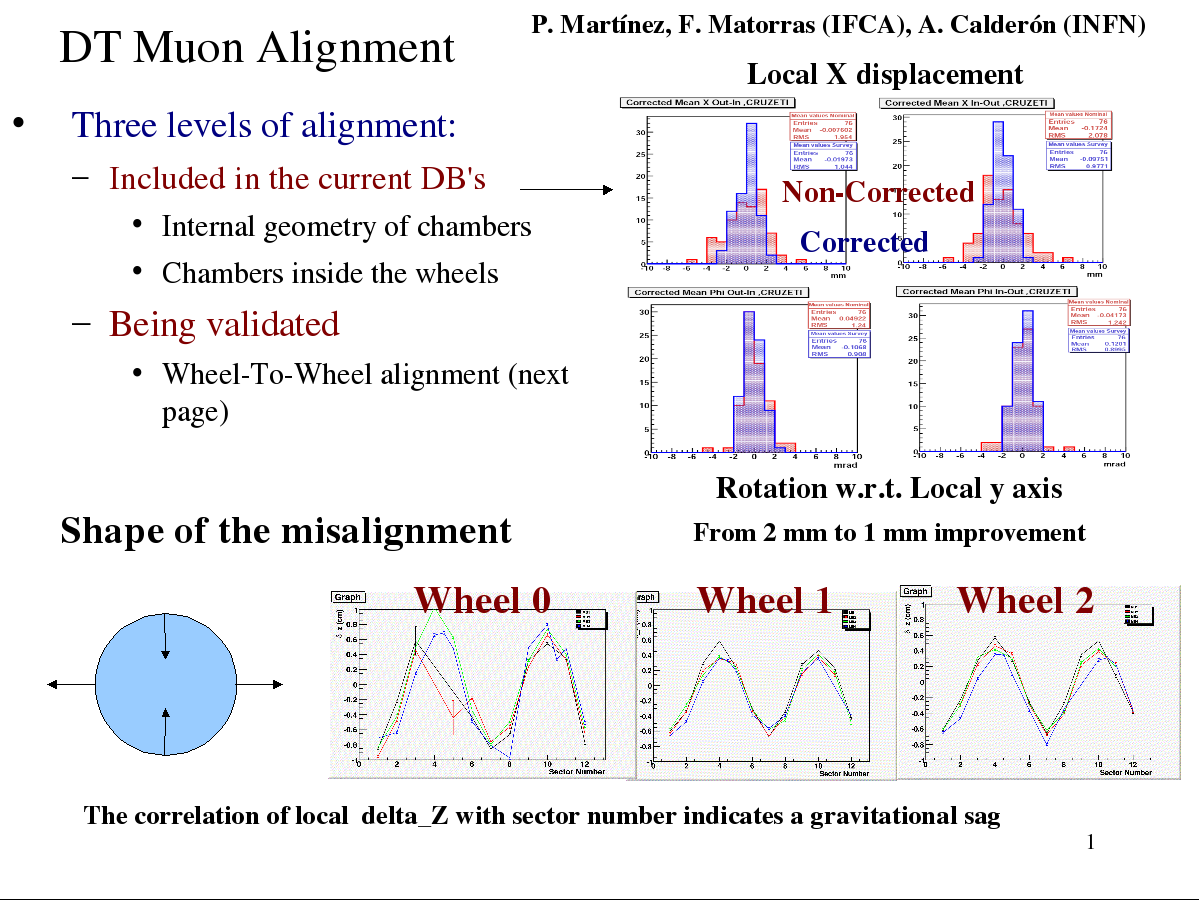
\includegraphics[width=1.2\linewidth]{Pablo1.png}}
\end{frame}

\begin{frame}
\mbox{\hspace{-1 cm}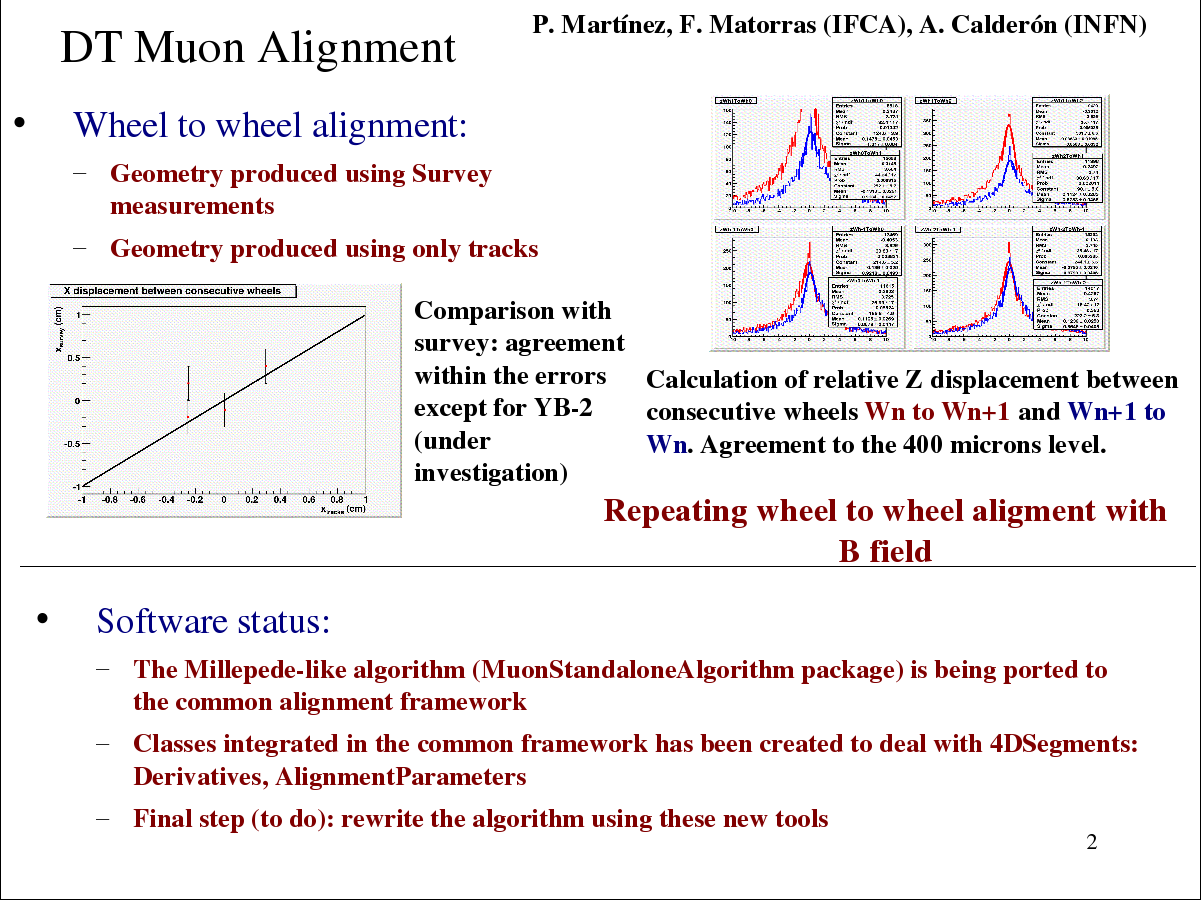
\includegraphics[width=1.2\linewidth]{Pablo2.png}}
\end{frame}

\section*{HIP and Endcap Alignments}
\begin{frame}
\begin{center}
\Huge \textcolor{blue}{HIP and Endcap Alignments}
\end{center}
\end{frame}

\begin{frame}
\frametitle{HIP-based program}
\small

\hspace{-0.5 cm} \begin{minipage}{\linewidth}
\begin{itemize}
\item Long-term plan is to fit muon track parameters to the tracker
  only and align muon chambers relative to fixed tracks
\begin{itemize}
\item uncorrelates objects on the same wheels, disks
\item yields tracker-muon interalignment
\end{itemize}
\item However,
\begin{itemize}
\item depends on tracker alignment unless \mbox{tracking volume sufficiently\hspace{-1 cm}}
  averaged over (e.g.\ with cosmic rays: see CSA08 results)
\item we should not wait for a large collisions sample to start!
\end{itemize}
\item Short-term plan:
\begin{itemize}
\item Take advantage of overlapping edges of CSCs to \mbox{align rings (this talk)\hspace{-1 cm}}
\item Align rings to tracker or muon barrel as rigid bodies with HIP

\vspace{0.1 cm} Demonstrated last CMS Week, we have since followed the
movement of CSC disks through all opening and closing and published result
in the database for CRUZET reprocessing
\end{itemize}

\item Medium-term plan:
\begin{itemize}
\item Align chambers to tracker in CRUZET-3/4 or CRAFT (better)
\end{itemize}
\end{itemize}
\end{minipage}
\end{frame}

\begin{frame}
\frametitle{CSC overlaps alignment}
\small

\begin{columns}
\small
\column{0.8\linewidth}
\begin{itemize}
\item Locally reconstruct tracks through \mbox{overlapping CSC edges\hspace{-1 cm}}
\item Essentially no multiple scattering, but sensitive to small effects (no averaging over a large volume)
\item Need to reconstruct whole ring of alignment corrections $A_i$ from pairwise residuals $\alpha_{i, i+1}$
\end{itemize}
\column{0.18\linewidth}
\vspace{0.5 cm}
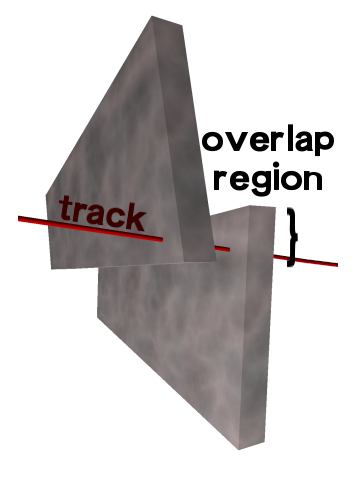
\includegraphics[width=\linewidth]{overlaps.png}
\end{columns}

\begin{itemize}
\item Methods:
\begin{itemize}
\item Propagate one at a time: simple diagnostic, but \mbox{error is cumulative\hspace{-1 cm}}
\item Iterate many times: generates 1-D waves (can be dampened)
\item Solve for global best-fit: only an 18$\times$18 or 36$\times$36 matrix
\end{itemize}
\end{itemize}

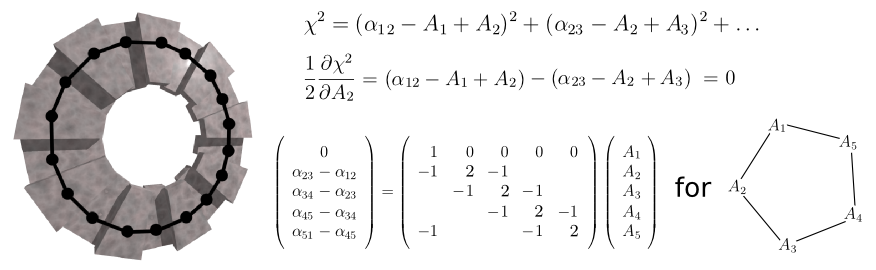
\includegraphics[width=\linewidth]{matrix_description_onestation.png}
\end{frame}

%% \begin{frame}
%% \frametitle{Evolution of procedure}
%% \small

%% \vspace{0.3 cm}
%% {\scriptsize
%% Began in February with HIP iterations, alternating between even and odd chambers
%% \begin{itemize}
%% \item Rings exploded in Monte Carlo, \hfill \mbox{ } \\
%% \mbox{ } \hfill due to too many free parameters, \hfill \mbox{ } \\
%% \mbox{ } \hfill reduced to 1-D (sometimes testing 2-D)
%% \item Diverged along straight lines, \hfill \mbox{ } \\
%% \mbox{ } \hfill due to poor two-chamber fits from full track fitter \hfill \mbox{ } \\
%% \mbox{ } \hfill replaced with linear fits
%% \item Discovered weak mode, \hfill \mbox{ } \\
%% \mbox{ } \hfill due to cancellation between left and right sides \hfill \mbox{ } \\
%% \mbox{ } \hfill replaced with one-sided fits
%% \item Ring seriously overclosed, \hfill \mbox{ } \\
%% \mbox{ } \hfill due to granularity of wire measurement, \hfill \mbox{ } \\
%% \mbox{ } \hfill replaced with a pure strip measurement
%% \item Rings moderately overclosed, \hfill \mbox{ } \\
%% \mbox{ } \hfill due to only approximately-correct degree of freedom, \hfill \mbox{ } \\
%% \mbox{ } \hfill switched from local $x$ (18-agon) to global $r\phi$ (circle)
%% \item Closure perfect in MC!  But not in data, \hfill \mbox{ } \\
%% \mbox{ } \hfill due in part to uncorrected angles, \hfill \mbox{ } \\
%% \mbox{ } \hfill introduced slope correction and track-track residual
%% \item Still imperfect (but better) closure, \hfill due to\ldots? \hfill \hfill \hfill \mbox{ } \\
%% \mbox{ } \hfill observe problem in independent ways, \mbox{overconstrain to isolate problem chambers\hspace{-0.3 cm}}
%% \end{itemize}}
%% \end{frame}

\begin{frame}
\frametitle{Evolution of procedure}
\small
\begin{itemize}
  \item Plan in February: HIP iterations, alternating even and odd chambers
  \item Given few observables, reduced to 1D (local $x$) for better control
  \item Switched from full tracker to linear fits, again for better control
  \item Discovered a weak mode due to cancellation between left and
    right side of chamber; dropped hits from one side (used other side
    as cross-check)
  \item Removed discretization effects from wire granularity by
    parameterizing alignment in global $r\phi$, rather than local $x$
  \item Solve whole-ring alignment in one step to speed up convergence
  \item Algorithm works very well in Monte Carlo!  (accurate, ring closes)
  \item But in data, there were still some effects
\begin{itemize}
  \item Misalignment angles are significant, switched from a track fit
    on one side to track fits on both sides to be sensitive to
    relative angles
  \item Observe system with as many different data-driven methods as
    possible for confidence
\end{itemize}
\end{itemize}
\end{frame}

\begin{frame}
\frametitle{Alignment with beam-halo}
\small

\begin{itemize}
\item On September 12, dataops delivered an AlCaReco sample of 110,000
  overlaps events and 825,000 generic beam-halo, reduced to tracks and
  hits for optimized reading
\item Armed with a working procedure in Monte Carlo, we went to work
  on the data immediately
\item The rest of this talk will show a snapshot of alignment status
  and current best results
\end{itemize}

\vfill
\hspace{-0.83 cm} \textcolor{darkblue}{\Large Parameters}

\vspace{0.2 cm}
\begin{columns}
\column{0.4\linewidth}
\begin{itemize}
\item $\varphi_y$ angles first,

then $r\phi$ positions
\item ME$-$2/1 \& ME$-$3/1 (highest statistics)
\item Run 62232: \mbox{2/3 of full \hspace{-0.5 cm}} statistics \mbox{in short time\hspace{-1 cm}}
\end{itemize}

\column{0.65\linewidth}
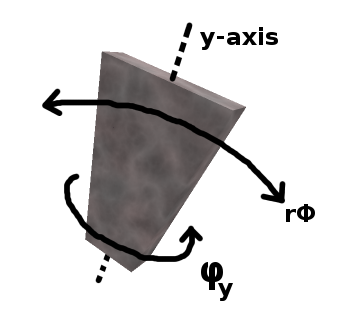
\includegraphics[width=0.38\linewidth]{one_chamber.png} 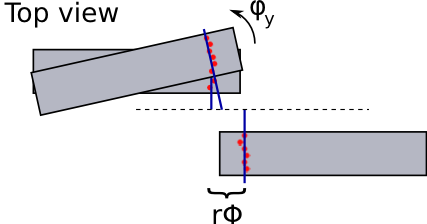
\includegraphics[width=0.62\linewidth]{order_of_parameters.png}
\end{columns}

\end{frame}

\begin{frame}
\frametitle{Determining $\varphi_y$ angles}
\small

Three independent methods (for cross-checks):
\begin{columns}
\column{0.6\linewidth}

\begin{enumerate}
\item Pure overlaps: $d\phi/dz$ slope must agree in pairs
\item Generic beam-halo: $d\phi/dz$ must agree on a track from ME$-$2/1 to ME$-$3/1
\item $d\phi/dz$ must be on average zero, because beam-halo tracks come from the LHC (absolute, not pairwise)
\end{enumerate}

\column{0.4\linewidth}
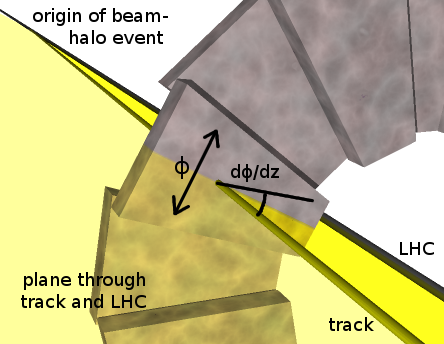
\includegraphics[width=\linewidth]{track_lhc_plane_closeup.png}
\end{columns}

\vspace{-0.2 cm}
\begin{columns}
\column{0.25\linewidth}
\begin{center}
Corrections from \textcolor{darkblue}{(1)} and \textcolor{darkblue}{(3)}:

\vspace{0.3 cm}
\scriptsize Completely different methods, disjoint sets of tracks, reproduces some trends

\end{center}
\column{0.65\linewidth}
\begin{center}
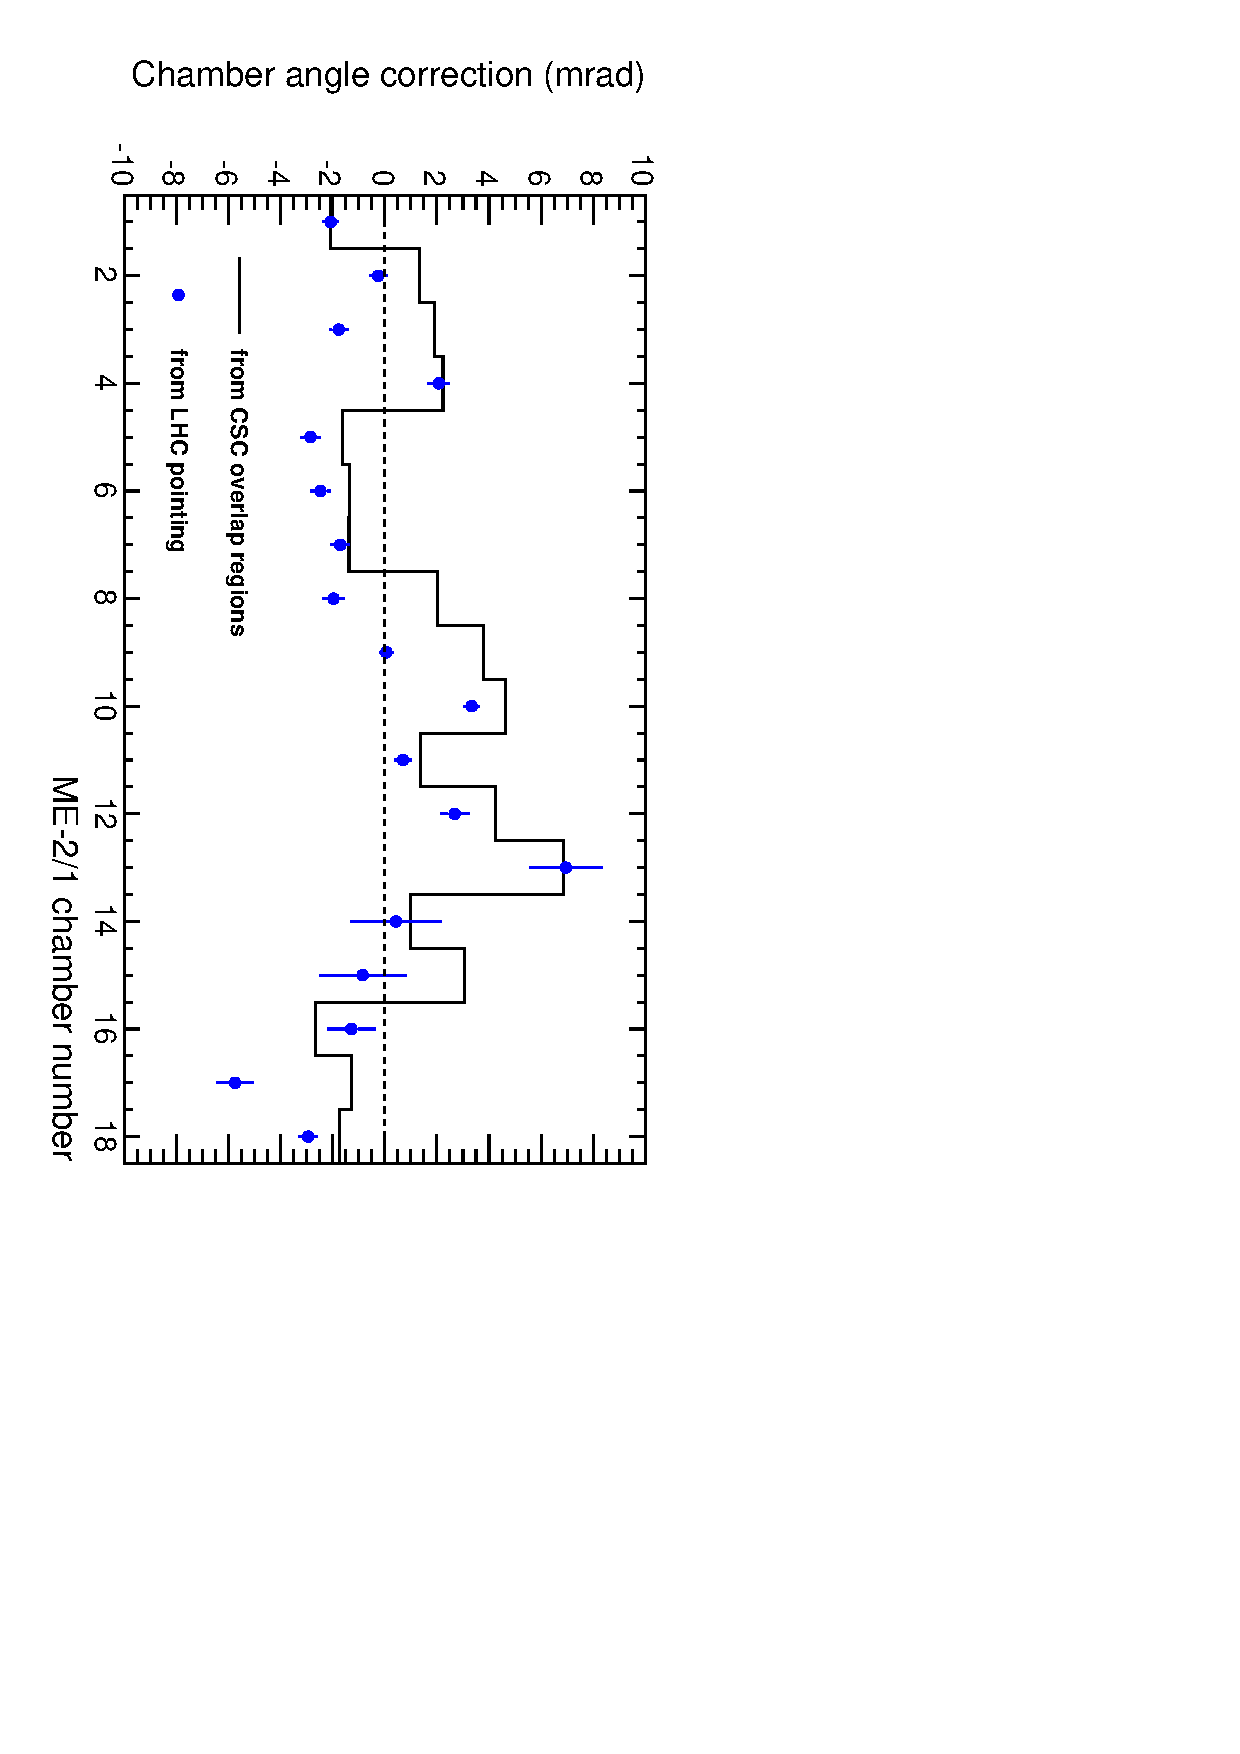
\includegraphics[height=\linewidth, angle=90]{angle_comparison_meminus21.pdf}
\end{center}
\end{columns}
\end{frame}

\begin{frame}
\frametitle{Determining $r\phi$ positions}
\small

Taking $\varphi_y$ from LHC pointing for now, we can attempt $r\phi$ alignment

\vspace{0.2 cm}
{\scriptsize (one needs a 10~mrad $\varphi_y$ misalignment to make a 1.25~mm mistake in $r\phi$, and we saw at most 4~mrad disagreements)}

\vfill
\begin{columns}
\column{0.4\linewidth}
Two independent methods:
\begin{enumerate}
\item Overlaps: track intercepts must match between $N$ and $N+1$
\item Straight-through: track must match between $N_{ME-2/1}$ and $N_{ME-3/1}$
\end{enumerate}

\column{0.65\linewidth}
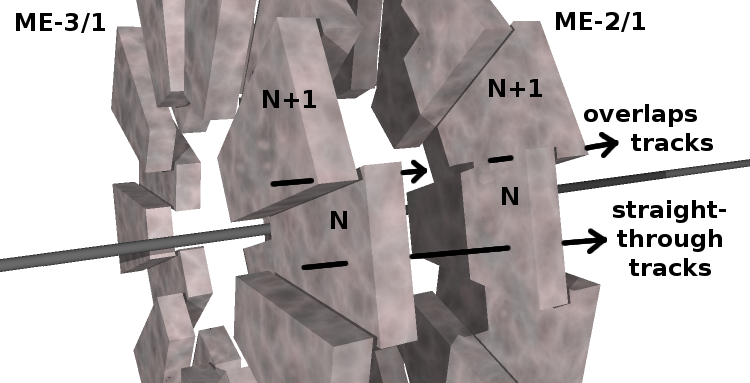
\includegraphics[width=\linewidth]{overlaps_straight_through.png}
\end{columns}

\vfill
Align with \textcolor{darkblue}{(1)} and look at a plot of \textcolor{darkblue}{(2)} for each $N$

(data-driven estimate of alignment quality)

\begin{itemize}
\item straight-through tracks pass through more material
\item but there are more of them
\end{itemize}
\end{frame}

\begin{frame}
\frametitle{Cross-checking $r\phi$ positions}
\small

\only<1>{\begin{itemize}
\item As we apply corrections, we improve alignment (as seen by straight-through tracks) in chambers 1--12 \& 18
\item Chambers 13--16 are unreliable due to poor statistics on $\varphi_y$
\end{itemize}}
\only<2>{\begin{itemize}
\item Don't attempt to align $\varphi_y$ on chambers 13--16 (leave at

default value) and repeat
\end{itemize}}

\begin{center}
\only<1>{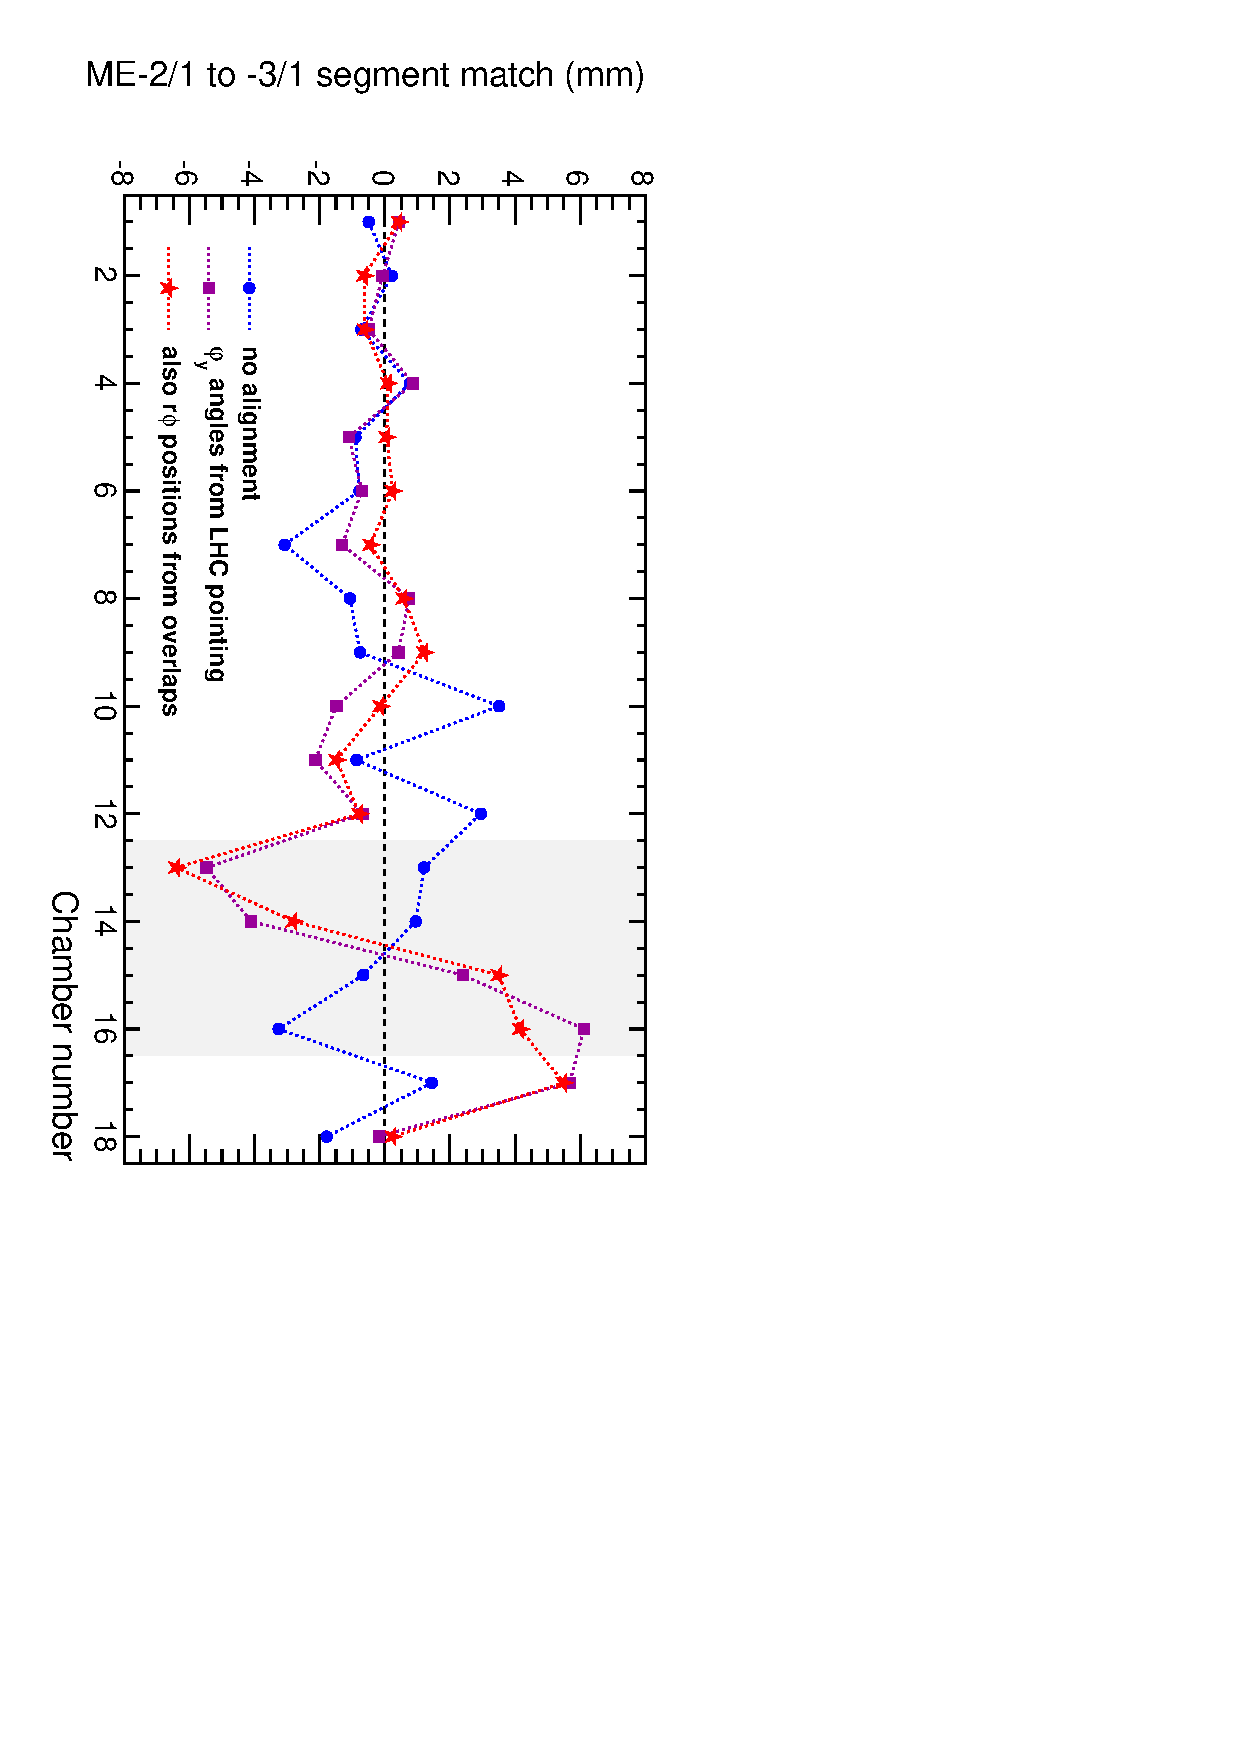
\includegraphics[height=0.75\linewidth, angle=90]{track_matching_better.pdf}}
\only<2>{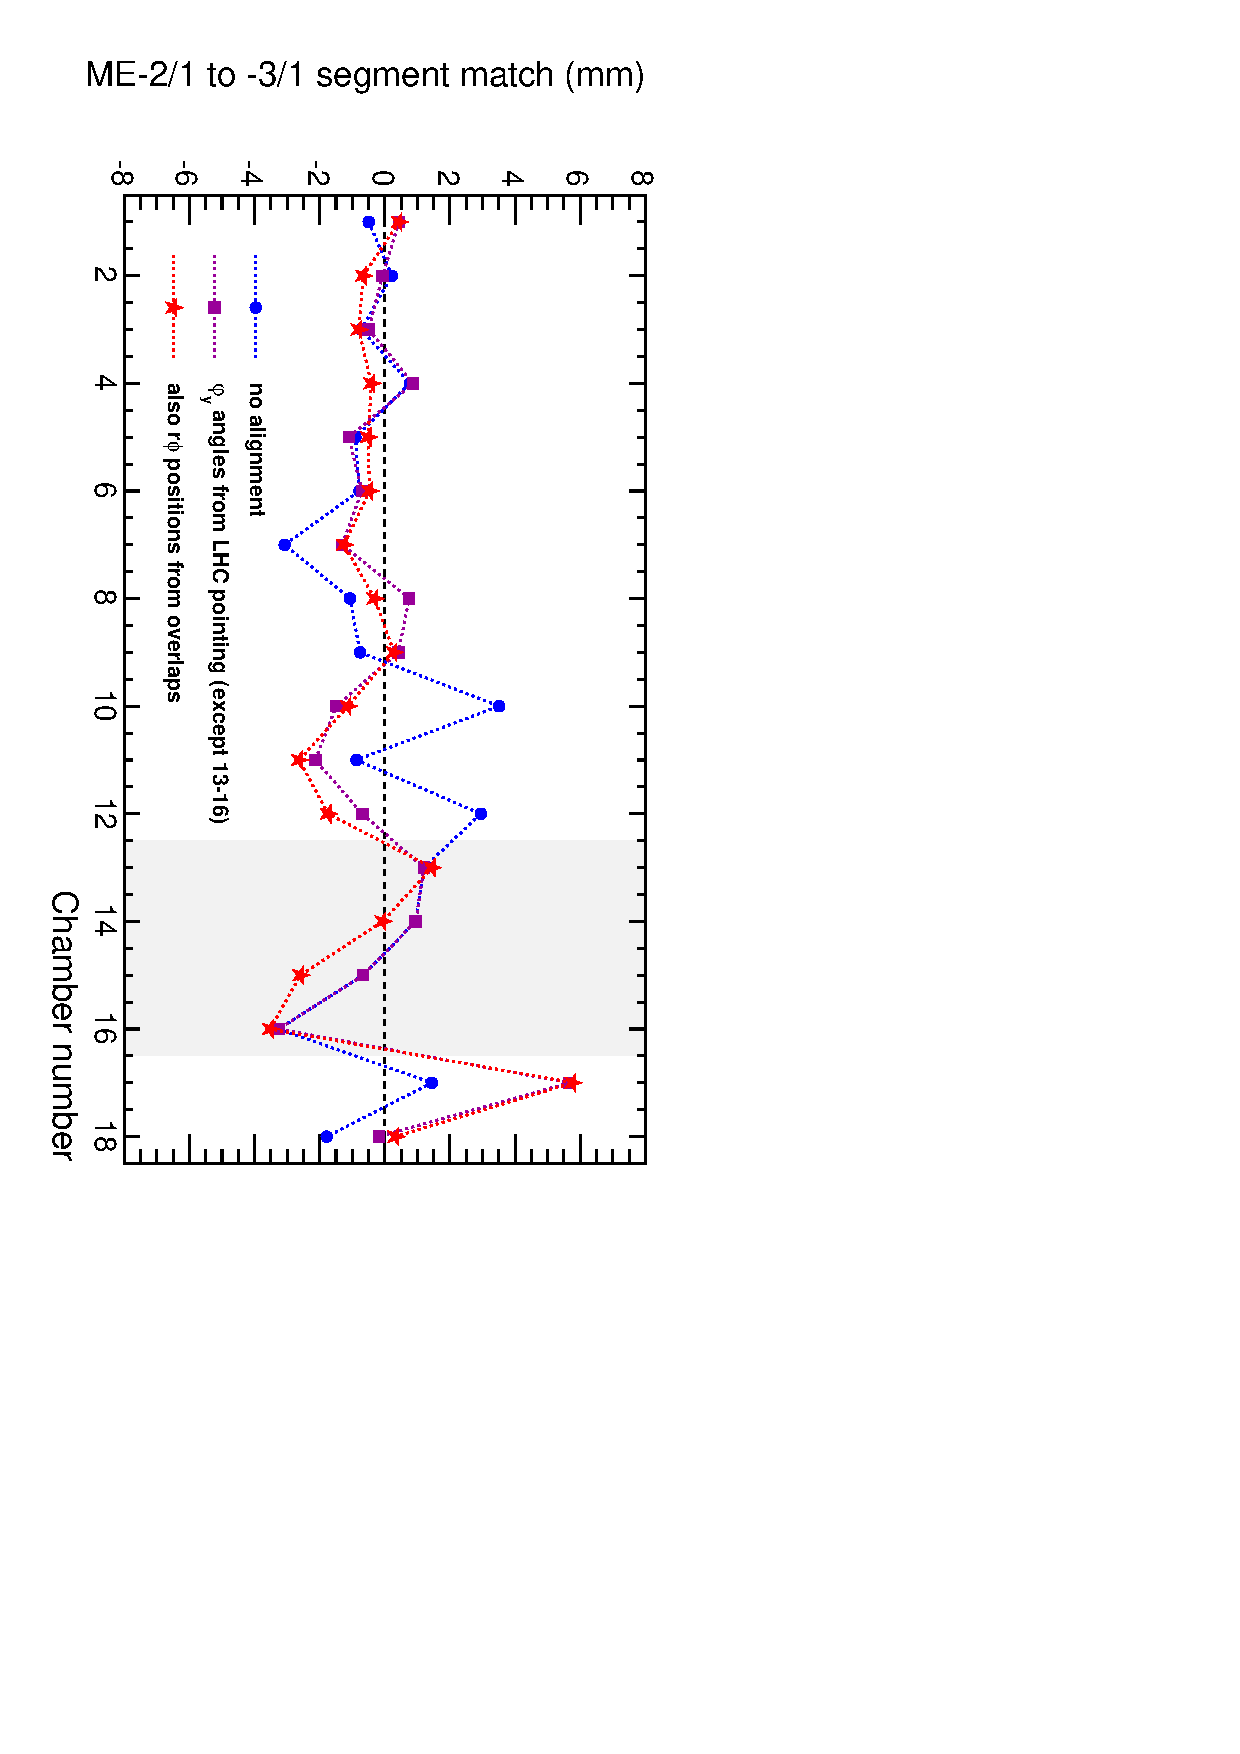
\includegraphics[height=0.75\linewidth, angle=90]{track_matching_better2.pdf}}

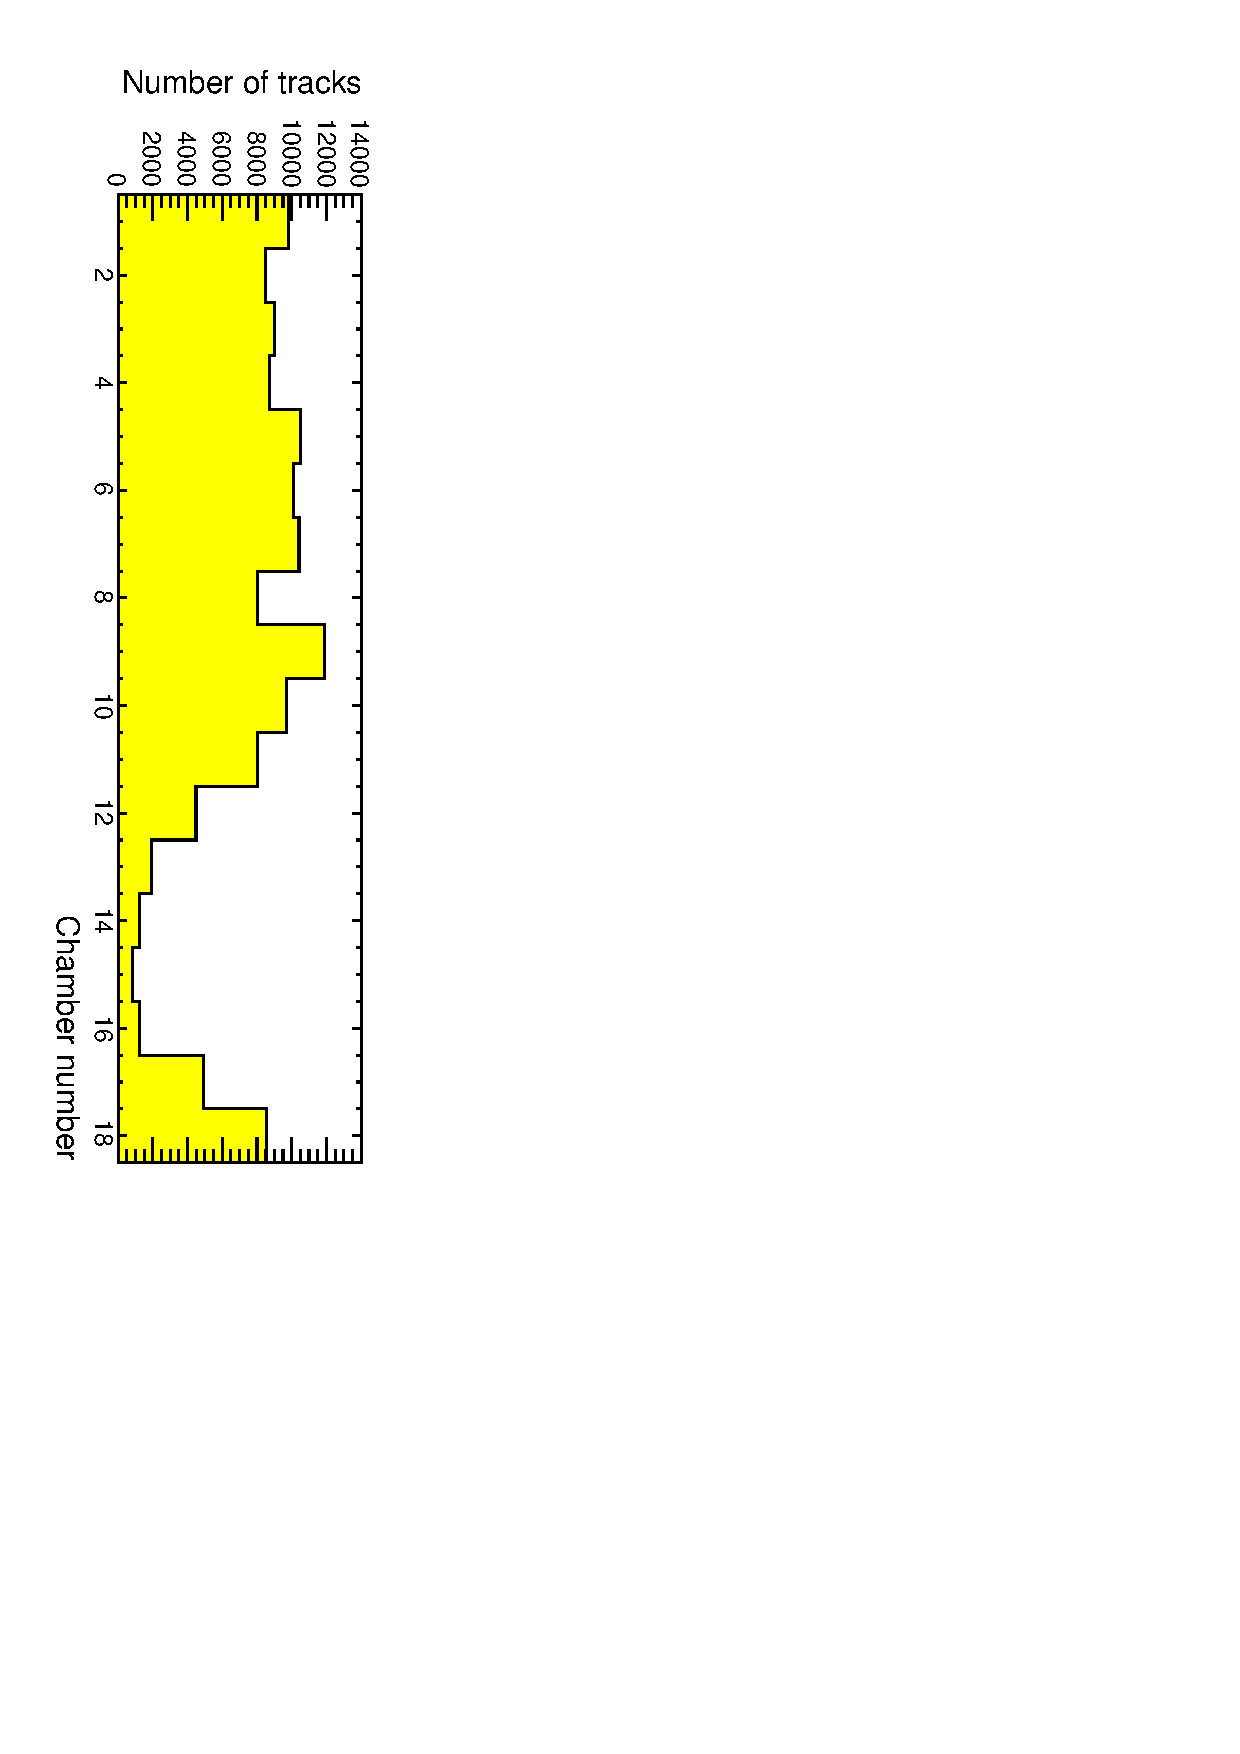
\includegraphics[height=0.75\linewidth, angle=90]{statistics.pdf}
\end{center}
\end{frame}

\begin{frame}
\frametitle{Another tool: combined fit}
\small

\begin{itemize}
\item Overlaps and straight-through tracks form a rigid frame: if errors are
not correlated between the rings, a combined fit would isolate errors
to one chamber (single-ring fit tries to distribute error uniformly)
\item Two benefits:
\begin{itemize}
\item diagnostic tool for identifying which chambers don't fit
\item yields the best set of constants with our present knowledge (excluding outliers)
\end{itemize}
\item But lose an independent cross-check
\end{itemize}

\vfill
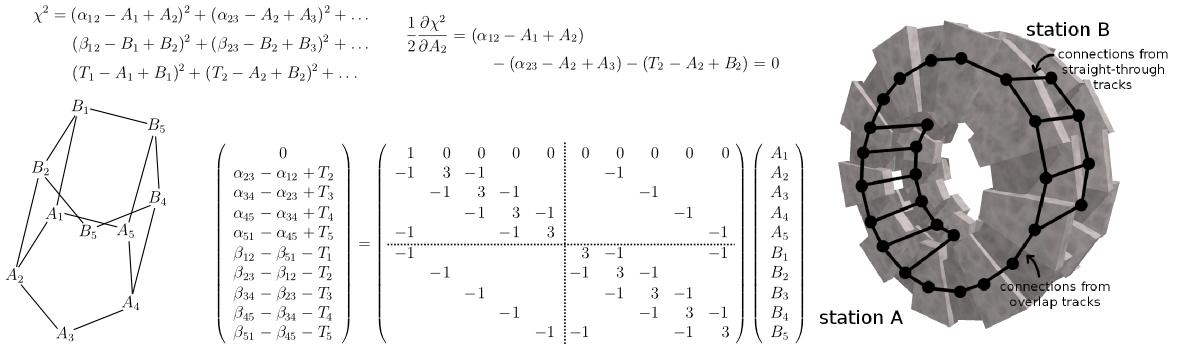
\includegraphics[width=\linewidth]{matrix_description.png}
\end{frame}

\begin{frame}
\frametitle{Example diagnostic}
\small

\hspace{-0.5 cm} Overlap residuals from combined fit (red line is single-ring fit, \mbox{grey is unaligned)\hspace{-1 cm}}

\vfill
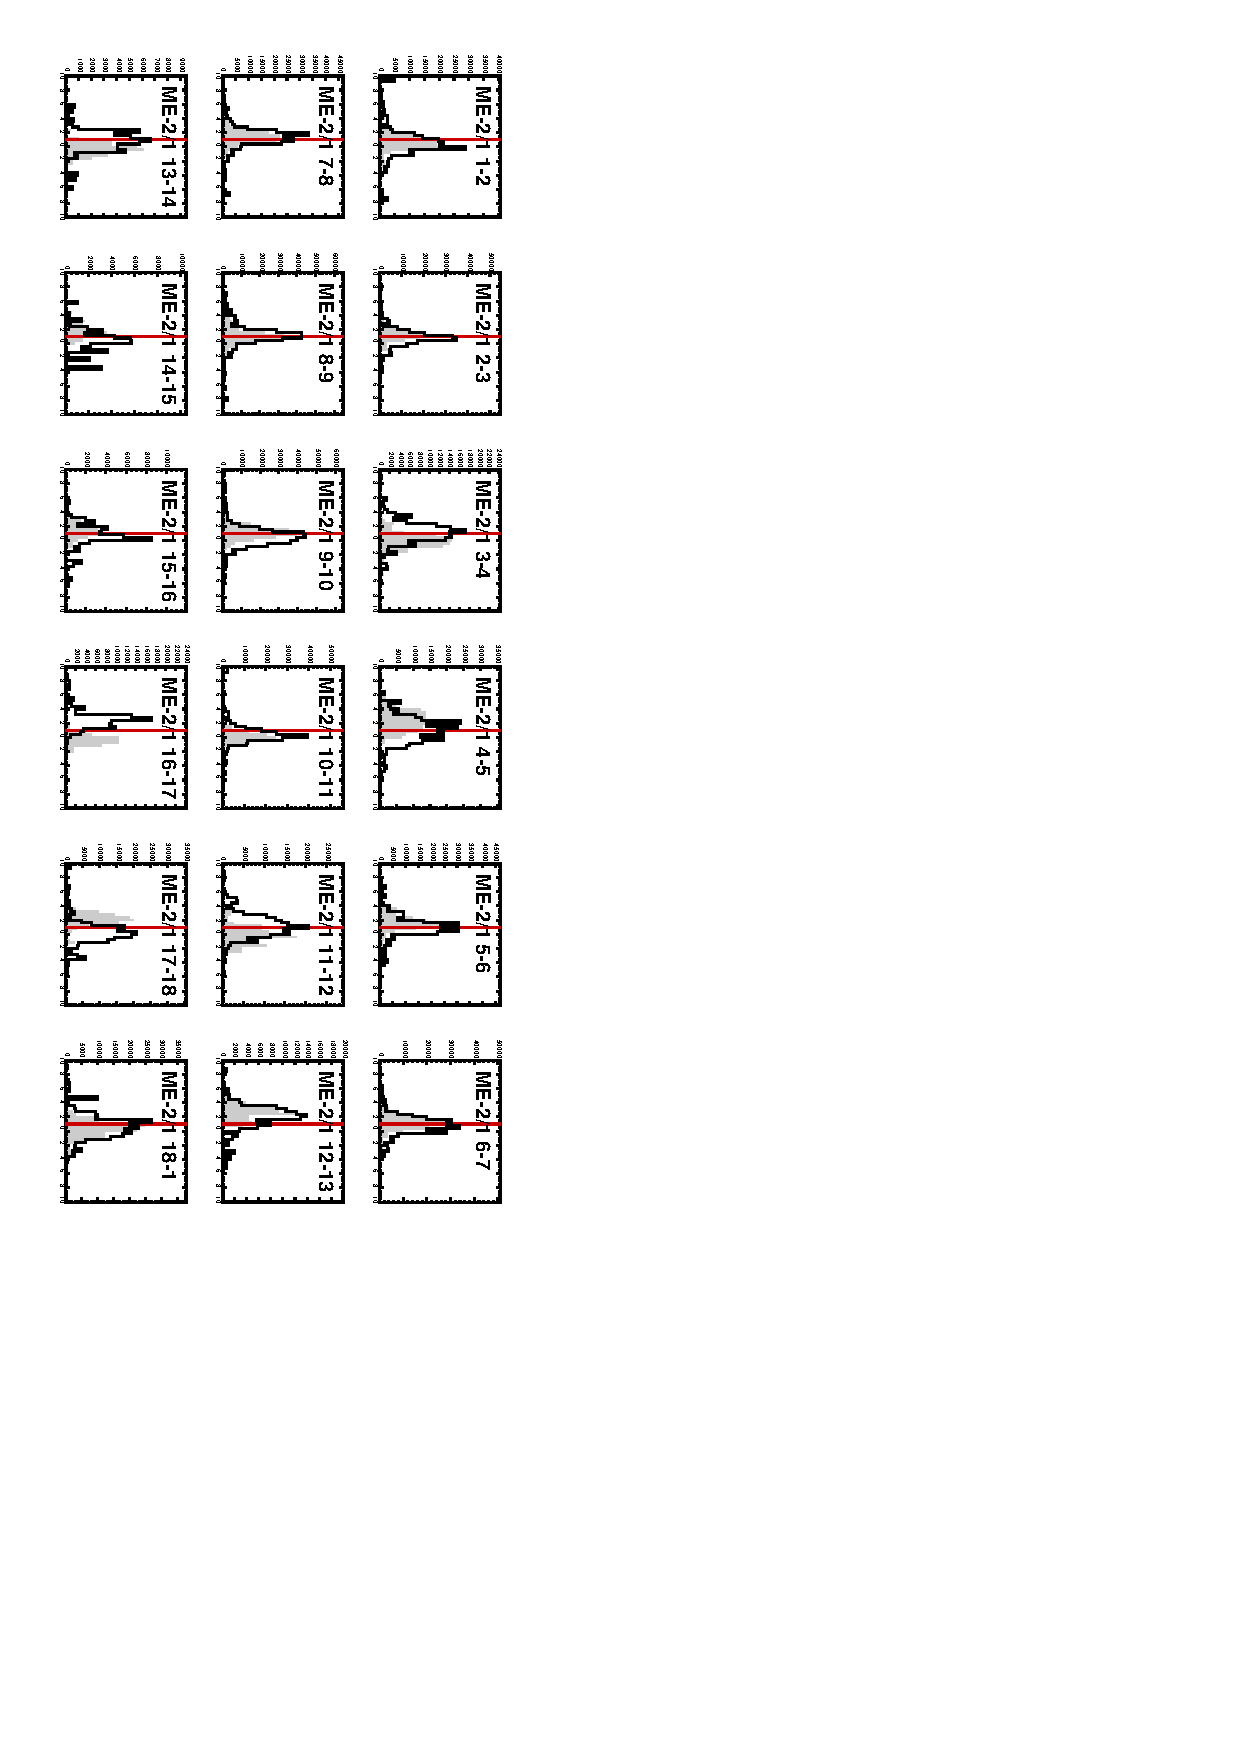
\includegraphics[height=\linewidth, angle=90]{final_checkresids_half.pdf}

\vfill
\begin{itemize}
\item Chamber 17 is clearly wrong (as we could have guessed from slide 14), also in ME$-$3/1, likely also a bad $\varphi_y$ angle
\item Also relevant to look at wide residuals vs.\ $y$ (for $\varphi_z$ rotation effects)
\end{itemize}
\end{frame}

\begin{frame}
\frametitle{Current best results}
\small
\begin{itemize}
\item Constants from combined fit with chambers 13--16 unrotated
\item Chamber 17 has the wrong angle in either ME$-$2/1 or ME$-$3/1
\item Chambers marked ``questionable'' also don't fit well
\item $\infty$-stats Monte Carlo resolution is 2.2~mrad in $\varphi_y$, 370~$\mu$m in $r\phi$
\end{itemize}

\begin{center}
\only<1>{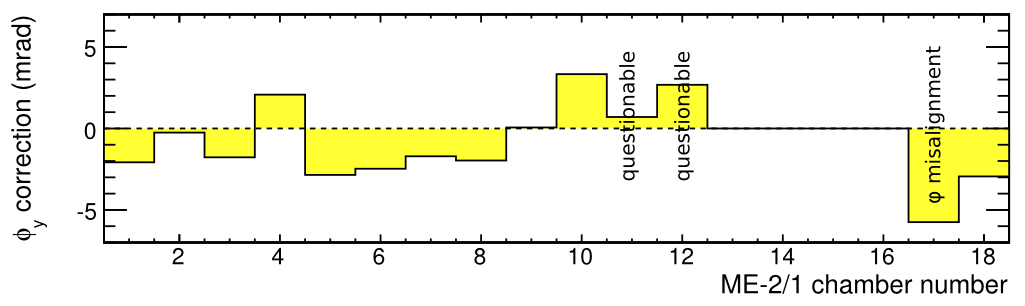
\includegraphics[width=0.9\linewidth]{present21_phiy.png}}
\only<2>{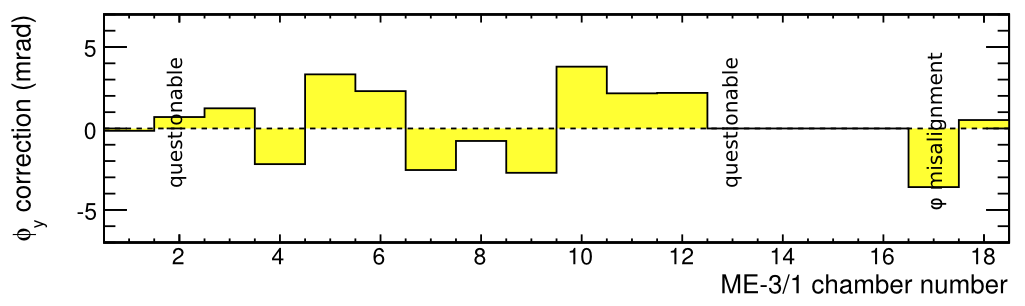
\includegraphics[width=0.9\linewidth]{present31_phiy.png}}

\only<1>{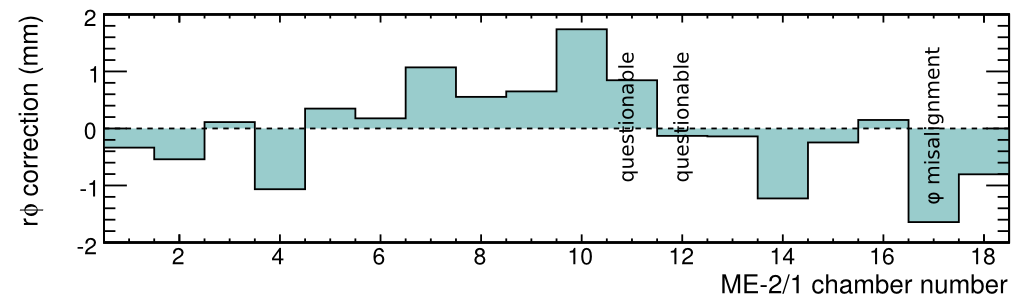
\includegraphics[width=0.9\linewidth]{present21_rphi.png}}
\only<2>{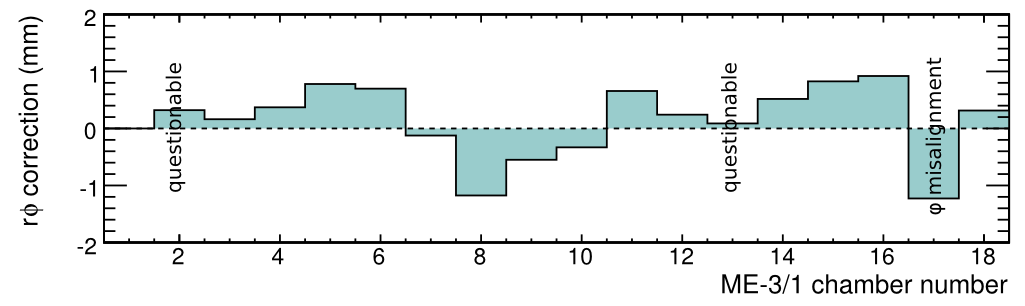
\includegraphics[width=0.9\linewidth]{present31_rphi.png}}
\end{center}
\end{frame}

\begin{frame}
\frametitle{Conclusions}

\begin{itemize}\setlength{\itemsep}{0.35 cm}
\item RMS of $r\phi$ constants is 750~$\mu$m, suggesting that the
  random error in both physical CSC placement and track-based
  alignment are small (RMS of $\varphi_y$ is 2.5~mrad)

\item Beam-halo events provide several different cross-checks on
  alignment (all with different systematics), in addition to
  comparison with hardware alignment

\item Part of a two-step process in which internally-aligned rings can
  be set relative to a reference (barrel or tracker)

\item Rings must be complete (only ME$+$2/1, ME$+$3/2, ME$-$2/1, ME$-$2/2,
  ME$-$3/1) or augmented with hardware measurement

\item Still trying to get a deeper understanding of these residuals
  (the overconstrained systems are not perfectly satisfied)
\end{itemize}

\label{numpages}
\end{frame}

\end{document}
